\documentclass[a4paper,12pt]{article}

\usepackage[utf8]{inputenc}
\usepackage[T1]{fontenc}
\usepackage{amsmath}
\usepackage{booktabs}
\usepackage{graphicx}
\usepackage{geometry}
\geometry{margin=2.5cm}
\usepackage{xcolor}
\usepackage{listings}
\usepackage{hyperref}
\hypersetup{colorlinks=true, linkcolor=blue!50!black, urlcolor=blue!50!black}
\renewcommand{\tablename}{Tabela}
\renewcommand{\figurename}{Figura}
\renewcommand{\lstlistingname}{Código}

% ---------- Configuração do realce de sintaxe (C) ----------
\definecolor{codebg}{RGB}{247,247,247}
\definecolor{codekw}{RGB}{0,0,180}
\definecolor{codecomment}{RGB}{0,128,0}
\definecolor{codestring}{RGB}{163,21,21}
\definecolor{framecolor}{RGB}{200,200,200}

\lstdefinestyle{cstyle}{
    language=C,
    backgroundcolor=\color{codebg},
    basicstyle=\ttfamily\footnotesize,
    keywordstyle=\color{codekw}\bfseries,
    commentstyle=\color{codecomment}\itshape,
    stringstyle=\color{codestring},
    numberstyle=\tiny\color{gray},
    numbers=left,
    numbersep=6pt,
    frame=single,
    rulecolor=\color{framecolor},
    breaklines=true,
    breakatwhitespace=false,
    showstringspaces=false,
    tabsize=4,
    captionpos=b,
    columns=flexible,
    morekeywords={size_t},
    extendedchars=true,
    literate=
        {á}{{\'a}}1 {à}{{\`a}}1 {â}{{\^a}}1 {ã}{{\~a}}1
        {é}{{\'e}}1 {ê}{{\^e}}1 {í}{{\'i}}1
        {ó}{{\'o}}1 {ô}{{\^o}}1 {õ}{{\~o}}1
        {ú}{{\'u}}1 {ü}{{\"u}}1 {ç}{{\c c}}1
        {Á}{{\'A}}1 {À}{{\`A}}1 {Â}{{\^A}}1 {Ã}{{\~A}}1
        {É}{{\'E}}1 {Ê}{{\^E}}1 {Í}{{\'I}}1
        {Ó}{{\'O}}1 {Ô}{{\^O}}1 {Õ}{{\~O}}1
        {Ú}{{\'U}}1 {Ü}{{\"U}}1 {Ç}{{\c C}}1
}

\title{Tarefa 12: Avaliação de Escalabilidade\\do Código de Navier-Stokes (OpenMP)}
\author{Israel Soares de Castro Filho \\ Matrícula: 20250070780}
\date{}

\begin{document}

\maketitle

\section{Introdução}

O objetivo desta tarefa é avaliar a escalabilidade do código de Navier-Stokes 2D
(apenas viscosidade, esquema explícito de 5 pontos, contorno periódico, malha
$1024 \times 1024$) em um nó de computação do NPAD, identificar os gargalos e
mostrar como cada versão do código mudou a escalabilidade da anterior.

\paragraph{Conceitos usados.}
\begin{itemize}
    \item \textbf{Desempenho} é a rapidez da execução ($1/T$).
          \textbf{Escalabilidade} é a eficiência com que usamos os recursos.
          Uma versão pode ser mais rápida e, ainda assim, escalar pior.
    \item \textbf{Speedup:} $S(p) = T(1)/T(p)$.
          \textbf{Eficiência:} $E(p) = S(p)/p$. Eficiência 100\% significa que
          os $p$ cores estão sendo totalmente aproveitados.
    \item \textbf{Escalabilidade forte:} o problema tem tamanho fixo e
          aumentamos os cores. O ideal é manter $E$ constante, mas a parte
          serial e os custos que não diminuem com $p$ (sincronização, memória)
          limitam isso (modelo de Amdahl).
    \item \textbf{Escalabilidade fraca:} o problema cresce junto com os cores
          (trabalho por core constante). O ideal também é manter $E$ constante
          (modelo de Gustafson).
    \item \textbf{Programa escalável:} é possível compensar a perda de
          eficiência causada por mais cores aumentando o tamanho do problema.
\end{itemize}

\section{Metodologia}

\paragraph{Ferramentas.} OpenMP para a paralelização, supercomputador NPAD
(um nó da partição \texttt{amd-512}, usado de forma exclusiva) e
\texttt{pascalanalyzer} com instrumentação manual, cujos relatórios foram
visualizados no PaScal Viewer.

\paragraph{Versões avaliadas.} A Tabela~\ref{tab:versoes} resume o que muda em
cada versão. Os trechos principais do código estão no Apêndice.

\begin{table}[h]
\centering
\begin{tabular}{@{}clll@{}}
\toprule
Versão & Mudança principal & Schedule & Região paralela \\
\midrule
1 & Paraleliza só o laço externo \texttt{i} & \texttt{runtime} & a cada passo \\
2 & \texttt{collapse(2)} nos laços \texttt{i} e \texttt{j} & \texttt{static} & a cada passo \\
3 & Laço interno sem condicionais + SIMD & \texttt{static} & a cada passo \\
4 & Uma única região paralela para todos os passos & \texttt{static} & única \\
\bottomrule
\end{tabular}
\caption{Versões do código. Na versão 1, o schedule foi variado por
\texttt{OMP\_SCHEDULE}: \texttt{static}, \texttt{dynamic,1}, \texttt{dynamic,16}
e \texttt{guided}.}
\label{tab:versoes}
\end{table}

\paragraph{Execução.} Cores: 1, 2, 4, 8, 16, 32 e 64. Seis entradas
(i1 a i6), com $t_{final}$ de 0,005 a 0,16, dobrando a cada entrada, o que
dobra o trabalho (número de passos), com $N = 1024$ fixo. Três repetições
por medição e threads fixadas aos cores
(\texttt{OMP\_PROC\_BIND=close}, \texttt{OMP\_PLACES=cores}). A região medida é
o passo de tempo; na versão 4, ela cobre todos os passos.

\paragraph{Como ler os heatmaps.} Cada linha é um número de cores (2 a 64) e
cada coluna é uma entrada (i1 a i6). No mapa de \emph{Efficiency}, escuro é
eficiência alta (próxima de 100\%) e claro é eficiência baixa. Nos demais, azul é
positivo e vermelho é negativo. Interpretamos a \emph{Strong Scalability} como
a evolução descendo uma coluna (mesma entrada, mais cores) e a
\emph{Weak Scalability} como avançar uma coluna dobrando os cores (trabalho por
core constante).

\section{Resultados}

As Figuras~\ref{fig:v1d1} a~\ref{fig:v4} mostram os heatmaps de cada
configuração e a Tabela~\ref{tab:resumo} resume a leitura deles.

\begin{table}[h]
\centering
\small
\begin{tabular}{@{}p{2.6cm}p{3.4cm}p{3.2cm}p{2.2cm}@{}}
\toprule
Versão & Eficiência com 2--8 cores & Onde a eficiência cai & Strong / Weak \\
\midrule
1, \texttt{dynamic,1} & Já abaixo das demais & A partir de 16 cores & Vermelho / vermelho \\
1, \texttt{dynamic,16} e \texttt{guided} & Alta (2--4 cores) & A partir de 16 cores & Vermelho / vermelho \\
1, \texttt{static} & Alta até 8--16 cores & Em 32--64 cores & Vermelho mais claro \\
2, \texttt{collapse} & Como a 1 \texttt{static} & Em 32--64 cores, um pouco depois & Vermelho mais claro \\
3, SIMD & Alta & Em 32--64 cores, parecida ou um pouco pior que a 2 & Vermelho mais claro \\
4, região única & Alta & Em 64 cores; melhor nas entradas maiores & Vermelho mais claro \\
\bottomrule
\end{tabular}
\caption{Resumo qualitativo dos heatmaps.}
\label{tab:resumo}
\end{table}

\begin{figure}[p]
\centering
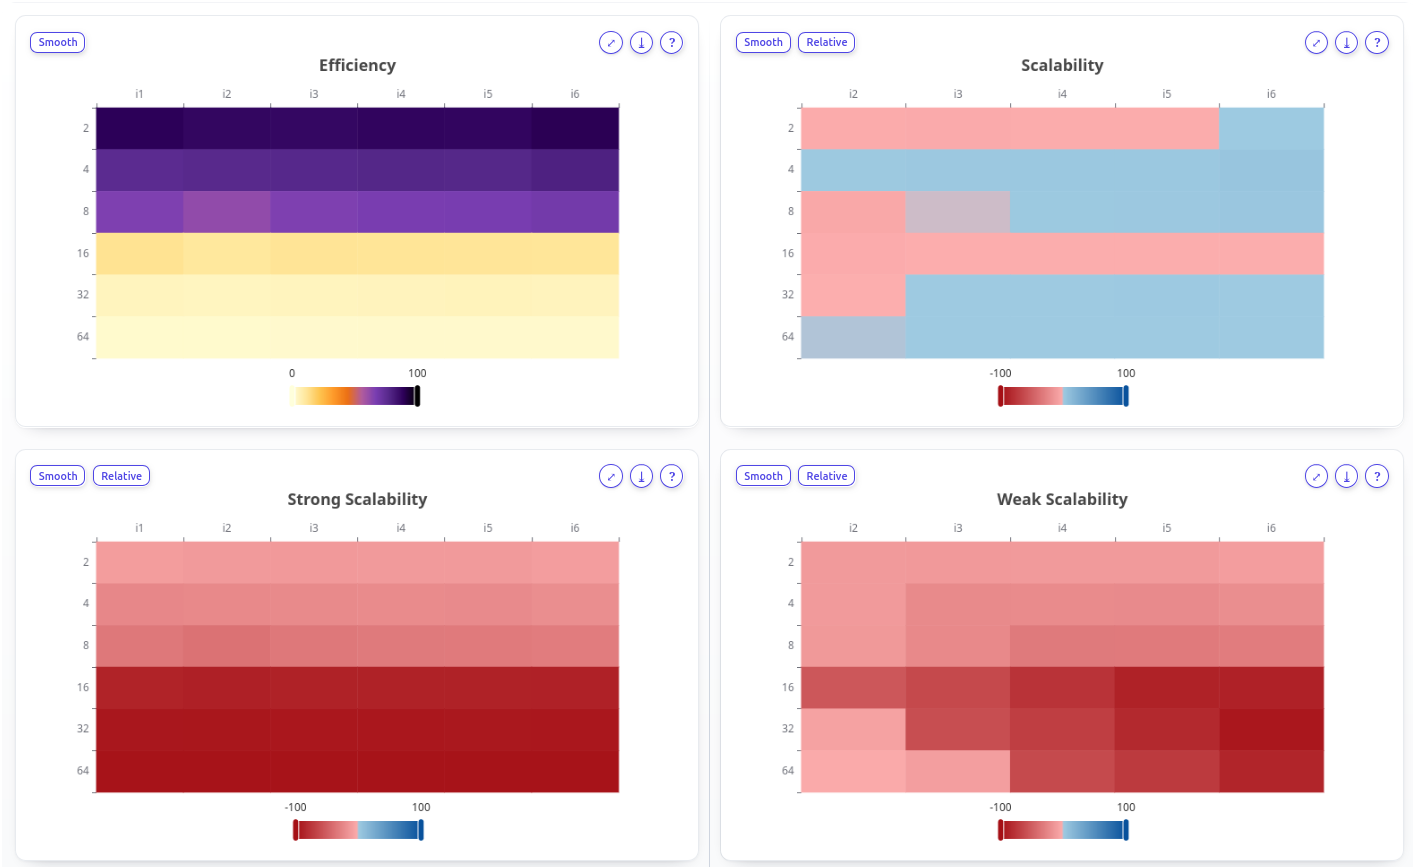
\includegraphics[width=0.95\textwidth]{../figuras/v1_dynamic-1.png}
\caption{Versão 1, \texttt{schedule(dynamic,1)}.}
\label{fig:v1d1}
\end{figure}

\begin{figure}[p]
\centering
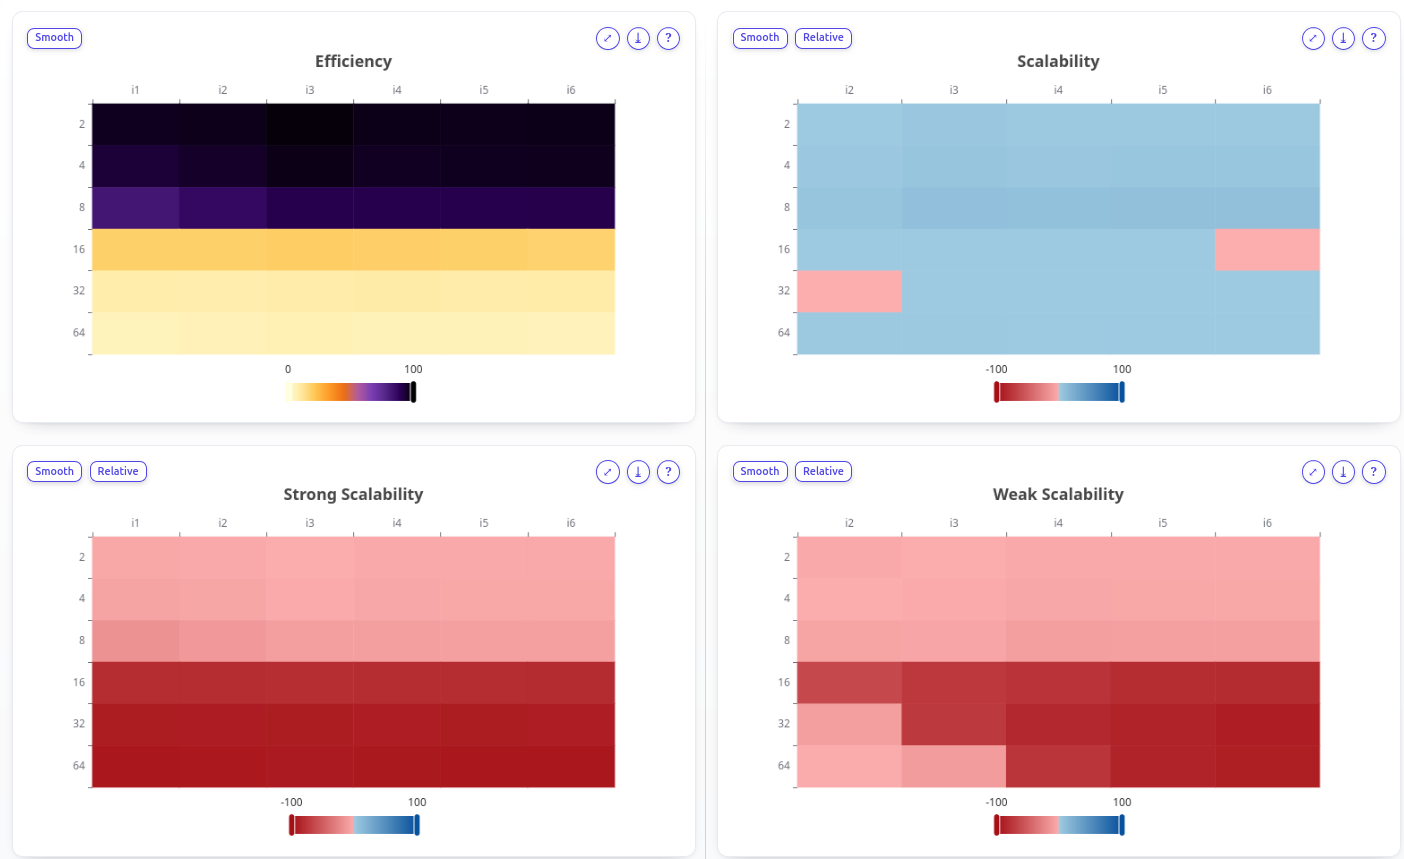
\includegraphics[width=0.95\textwidth]{../figuras/v1_dynamic-16.png}
\caption{Versão 1, \texttt{schedule(dynamic,16)}.}
\label{fig:v1d16}
\end{figure}

\begin{figure}[p]
\centering
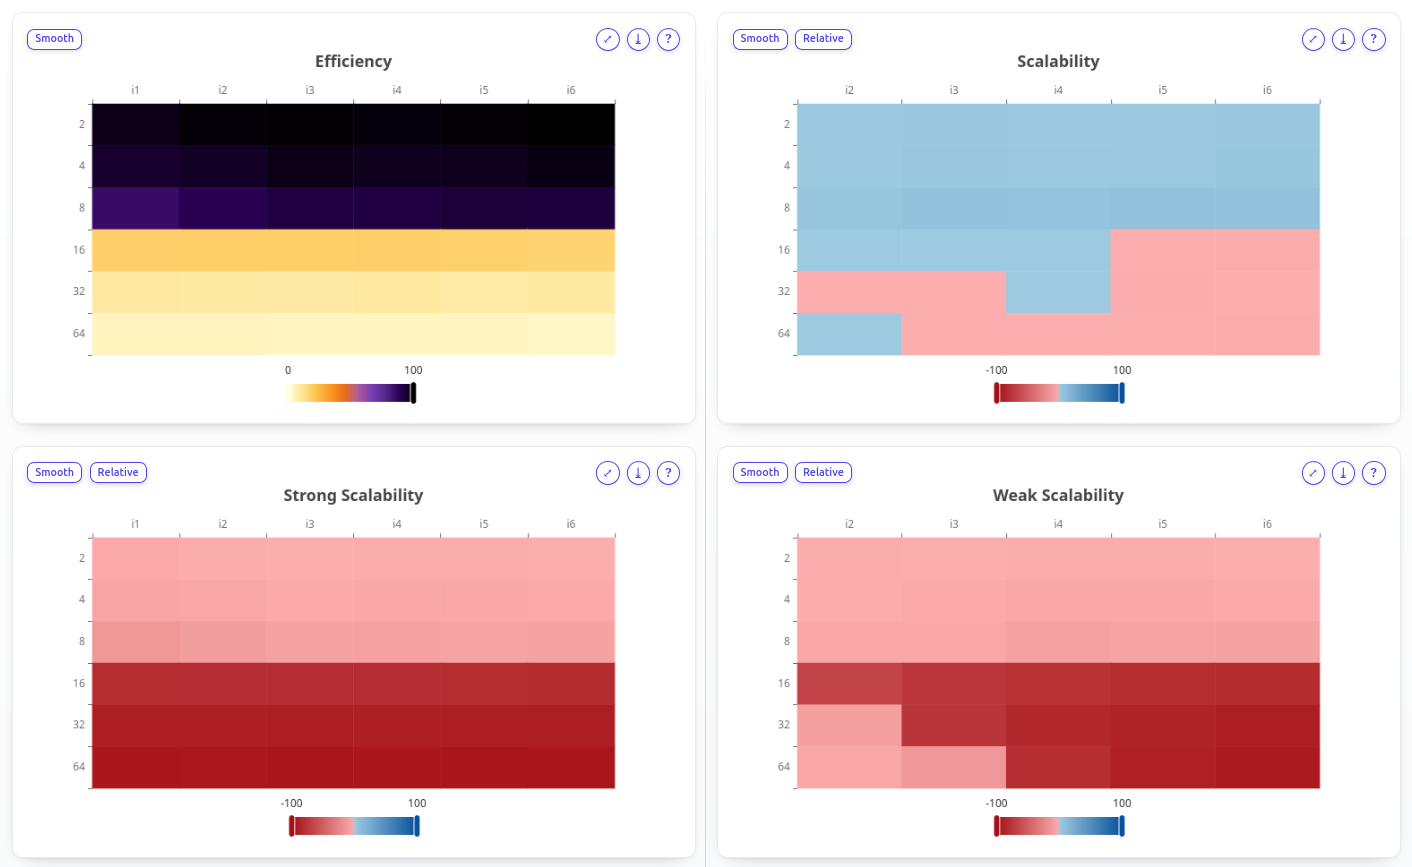
\includegraphics[width=0.95\textwidth]{../figuras/v1_guided.png}
\caption{Versão 1, \texttt{schedule(guided)}.}
\label{fig:v1g}
\end{figure}

\begin{figure}[p]
\centering
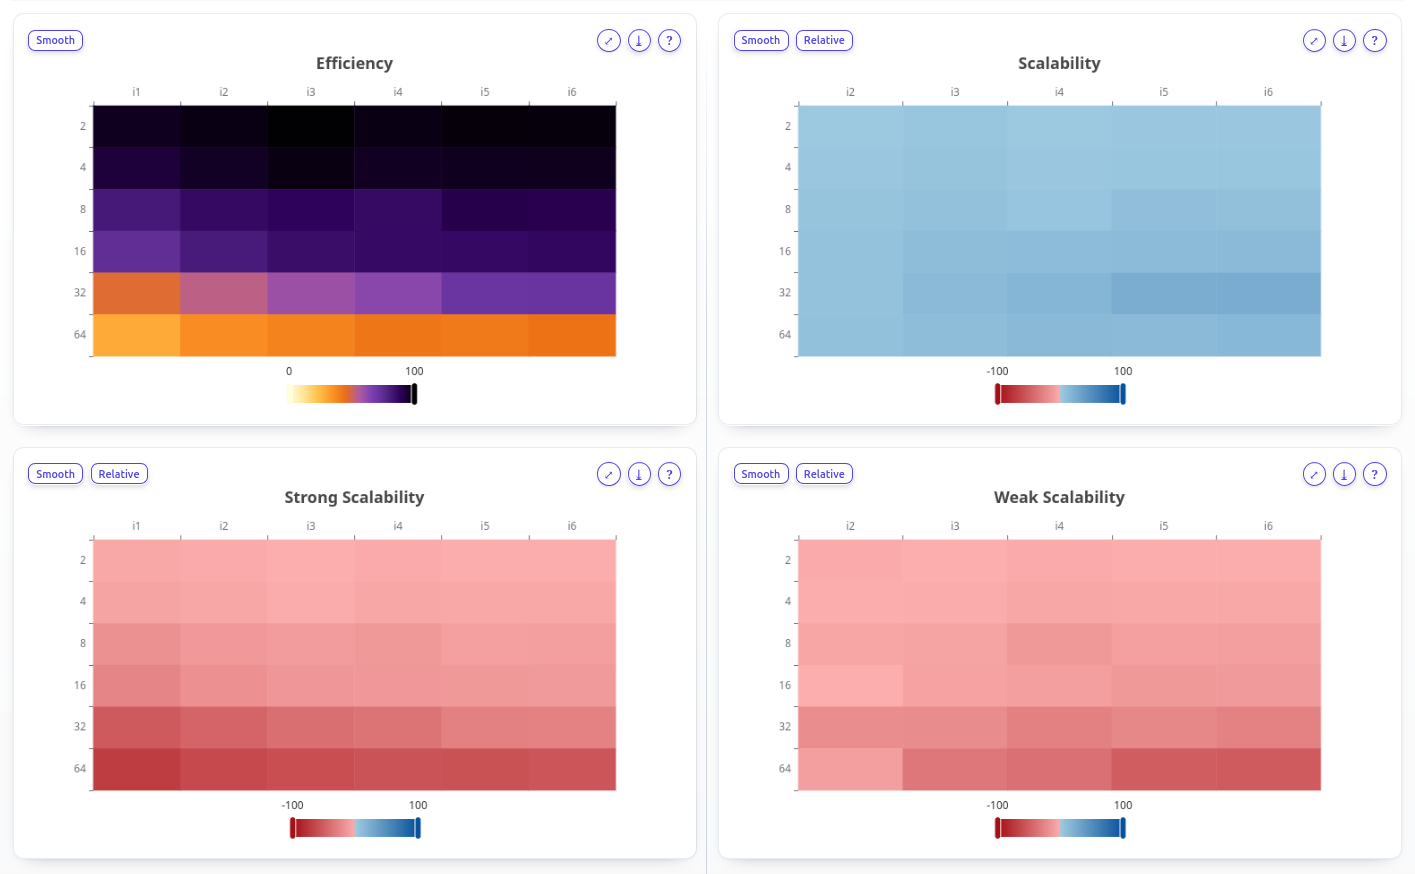
\includegraphics[width=0.95\textwidth]{../figuras/v1_static.png}
\caption{Versão 1, \texttt{schedule(static)}.}
\label{fig:v1s}
\end{figure}

\begin{figure}[p]
\centering
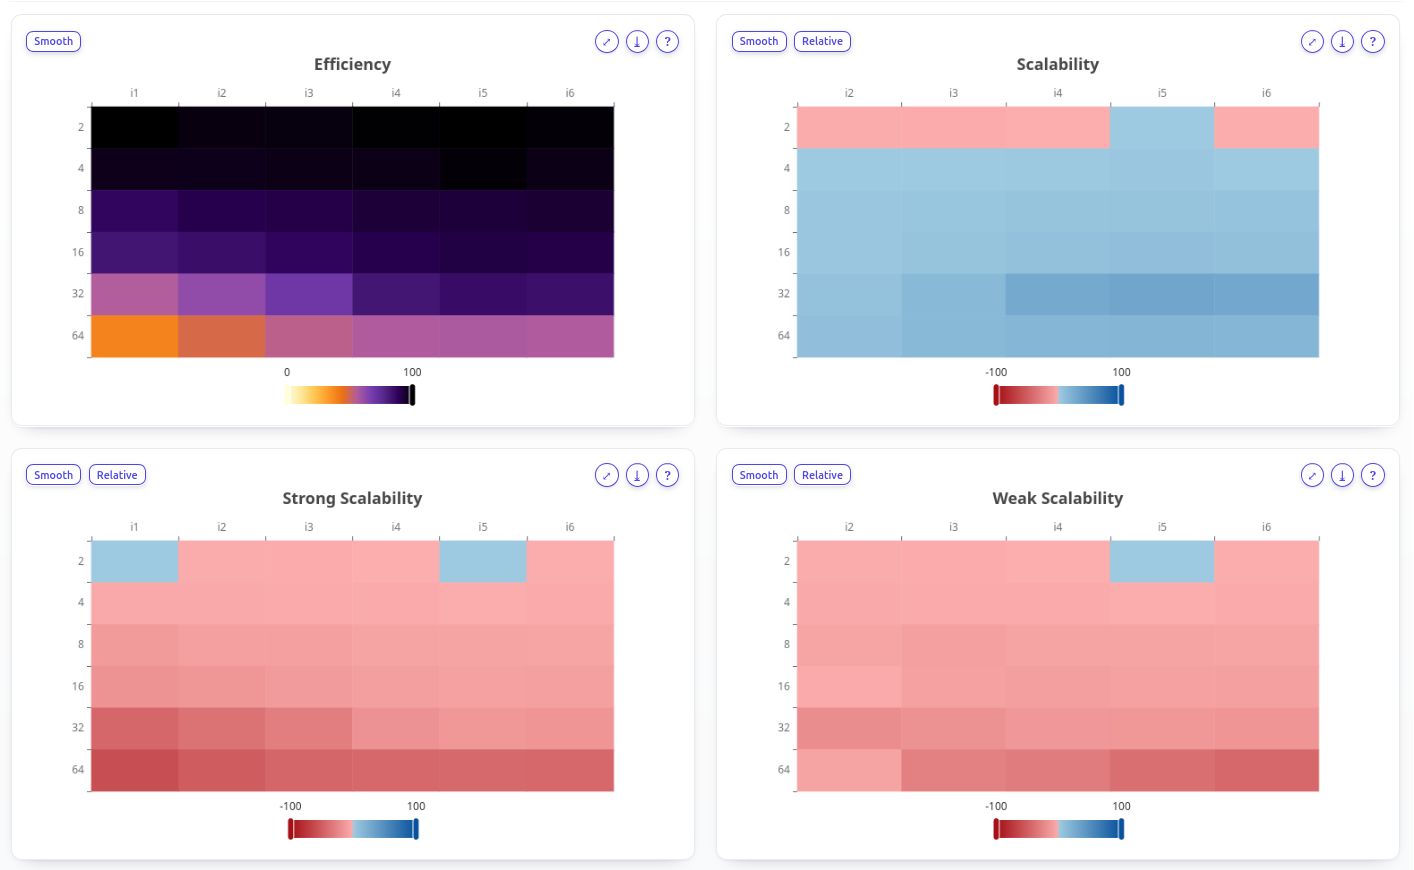
\includegraphics[width=0.95\textwidth]{../figuras/v2_collapse.png}
\caption{Versão 2, \texttt{collapse(2)} com \texttt{static}.}
\label{fig:v2}
\end{figure}

\begin{figure}[p]
\centering
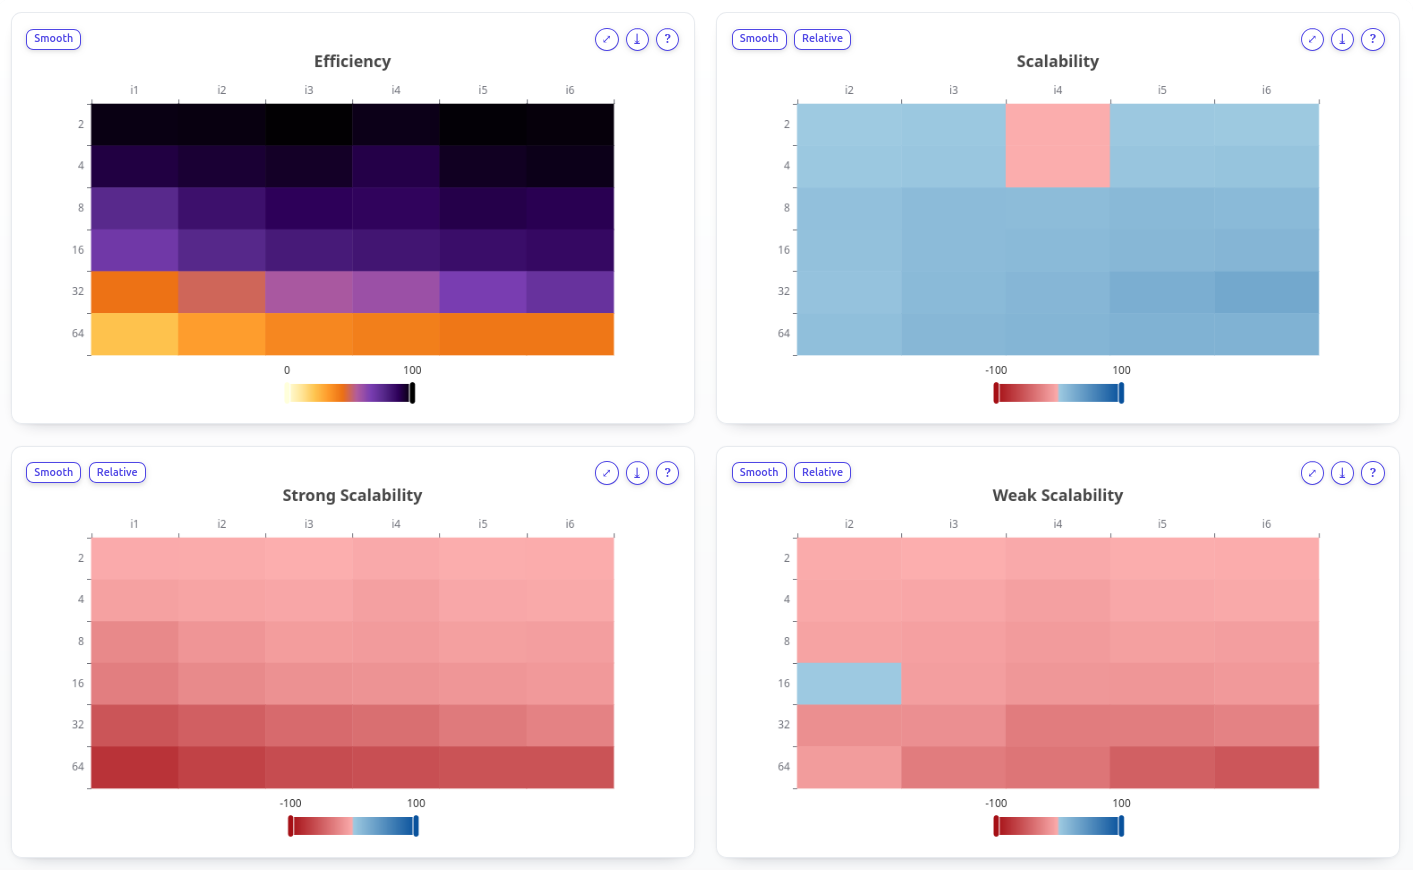
\includegraphics[width=0.95\textwidth]{../figuras/v3_simd.png}
\caption{Versão 3, laço sem condicionais e SIMD.}
\label{fig:v3}
\end{figure}

\begin{figure}[p]
\centering
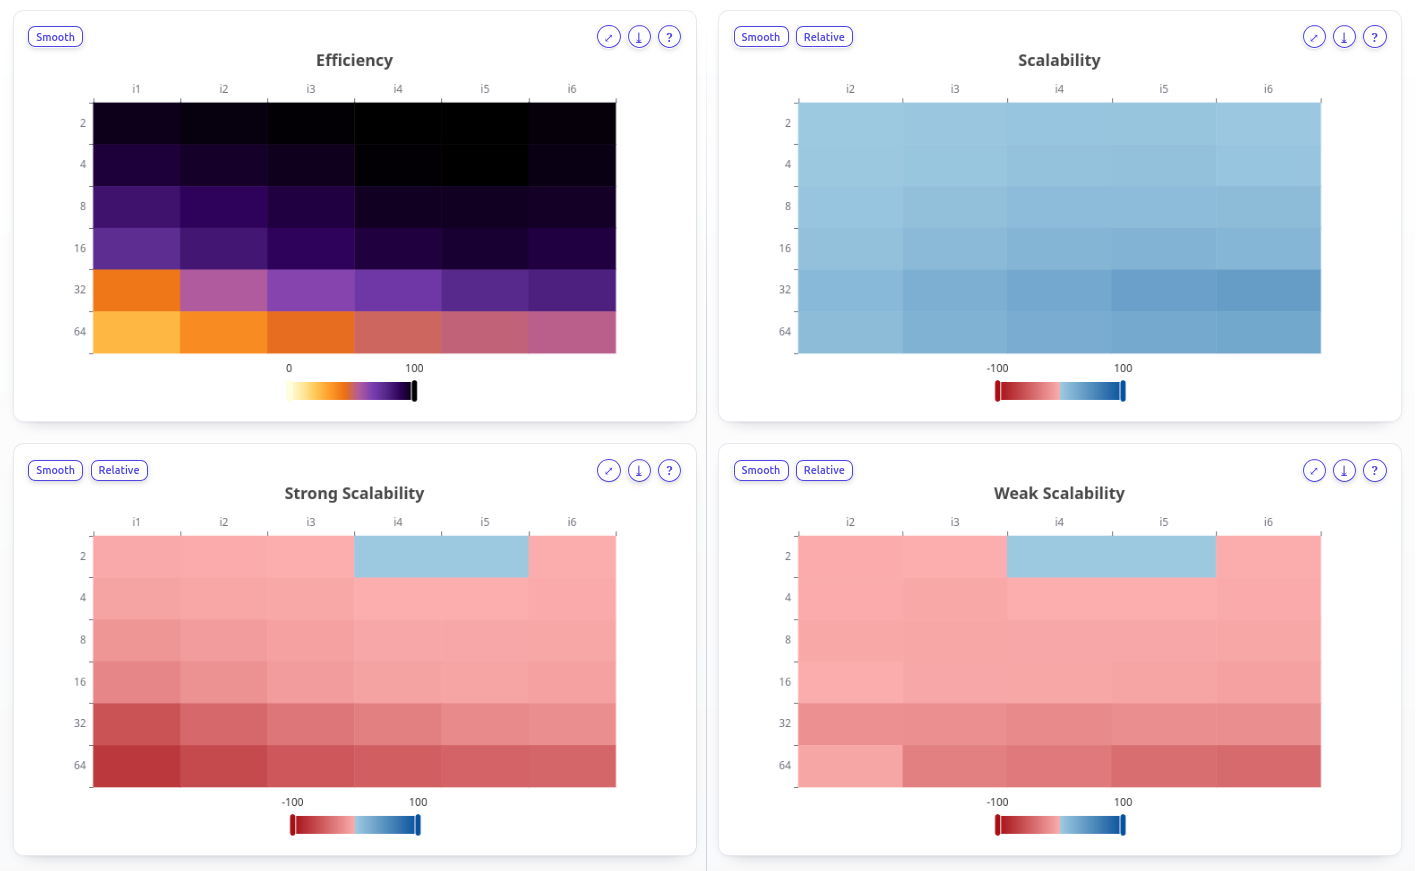
\includegraphics[width=0.95\textwidth]{../figuras/v4_regiao.png}
\caption{Versão 4, região paralela única.}
\label{fig:v4}
\end{figure}

\clearpage
\section{Análise}

\subsection{Versão 1: o schedule é o primeiro gargalo}

\textbf{Gargalos.} (i) O custo do escalonamento: com \texttt{dynamic} cada
thread busca iterações em uma fila compartilhada, o que custa mais quanto menor
o chunk, e a linha de uma thread muda de dono a cada passo, perdendo dados em
cache. (ii) Só o laço \texttt{i} é paralelo: são apenas 1024 iterações, ou
seja, 16 linhas por thread com 64 threads. (iii) Há uma região paralela (criação
da equipe e barreira) a cada passo de tempo.

\textbf{O que vemos.} Com \texttt{dynamic,1} a eficiência já é menor com poucos
cores (Figura~\ref{fig:v1d1}). \texttt{dynamic,16} e \texttt{guided} melhoram
com 2--4 cores, mas a eficiência despenca a partir de 16 cores
(Figuras~\ref{fig:v1d16} e~\ref{fig:v1g}). O \texttt{static}
(Figura~\ref{fig:v1s}) segura a eficiência por mais tempo, pois o custo por
linha é uniforme e não há o que balancear dinamicamente.

\textbf{Escalabilidade.} \emph{Forte:} ruim em todos os schedules (vermelho).
\emph{Fraca:} ruim com \texttt{dynamic} e \texttt{guided}. \emph{Programa escalável:} com
\texttt{dynamic} e \texttt{guided}, as linhas de 16 a 64 cores continuam claras até
a maior entrada, ou seja, aumentar o problema não recupera a eficiência. Com
\texttt{static}, a eficiência melhora para as entradas maiores.

\subsection{Versão 2: \texttt{collapse(2)}}

\textbf{Mudança.} Os laços \texttt{i} e \texttt{j} viram um só, com cerca de
$10^6$ iterações em vez de 1024, e o schedule passa a ser \texttt{static} fixo.

\textbf{Efeito.} O padrão é muito parecido com o da versão 1 \texttt{static}
(Figura~\ref{fig:v2}), com uma leve melhora em 32--64 cores. Mais iterações
ajudam a dividir o trabalho com muitos cores, mas o gargalo principal não era
o balanceamento. Continuam presentes a região paralela a cada passo e o
acesso à memória, e o código ainda recalcula os vizinhos com condicionais em
todo ponto.

\textbf{Escalabilidade.} Forte: ainda ruim, mas a queda vem mais tarde.
Fraca: parcial. A eficiência melhora nas entradas maiores.

\subsection{Versão 3: laço interno sem condicionais e SIMD}

\textbf{Mudança.} O miolo do laço interno ($j = 1, \dots, N-2$) não tem mais
condicionais de contorno, e as bordas são tratadas à parte, o que permite
vetorizar (\texttt{omp simd}). Também são usados ponteiros de linha em vez de
\texttt{IDX()} repetido.

\textbf{Efeito.} Essa mudança acelera a execução com 1 thread, mas o heatmap
fica parecido ou um pouco pior que o da versão 2 em 32--64 cores
(Figura~\ref{fig:v3}). Isso acontece porque a eficiência é medida contra o
tempo de 1 thread \emph{da própria versão}. Com a parte de cálculo mais rápida, os
custos que não diminuem com $p$ (barreira, criação da equipe, banda de
memória) pesam mais na proporção. Esse é um bom exemplo de
\emph{desempenho} melhorar sem a \emph{escalabilidade} melhorar.

\textbf{Escalabilidade.} Forte e fraca: semelhantes às da versão 2.

\subsection{Versão 4: região paralela única}

\textbf{Mudança.} A região \texttt{parallel} é criada uma vez, fora do laço de
tempo. Dentro dela, cada passo é um \texttt{omp for} com a barreira implícita,
que é necessária porque o passo $n+1$ depende do passo $n$. Os diagnósticos
também ficam dentro da mesma região.

\textbf{Efeito.} Elimina o custo de criar e encerrar a equipe de threads a cada
passo, o que importa quando cada thread tem pouco trabalho por passo. No heatmap
(Figura~\ref{fig:v4}), a versão 4 parece manter a eficiência um pouco melhor
com 64 cores nas entradas maiores, com ganho moderado. A eficiência com 64 cores
continua baixa. Os gargalos que sobram são a barreira a cada passo, a banda de
memória (o stencil faz poucas contas por dado lido) e a malha pequena
(16 linhas por thread).

\textbf{Escalabilidade.} Forte: continua não sendo fortemente escalável. Fraca e
programa escalável: a eficiência se recupera com entradas maiores, sendo a
melhor das versões nessa tendência.

\subsection{Observações sobre os resultados}

\begin{itemize}
    \item Neste experimento, aumentar a entrada aumenta o número de passos, não
          o tamanho da malha. A melhora com entradas maiores vem de diluir
          custos fixos (alocação, inicialização, saída) e não de mais
          paralelismo por passo. 
    \item Para avaliar escalabilidade fraca de forma
          mais fiel, é preciso variar o tamanho $N$ da malha.
\end{itemize}

\section{Conclusão}

Nenhuma das versões é fortemente escalável: com $N=1024$ fixo, a eficiência cai
quando os cores aumentam. O que mudou entre as versões foi \emph{onde} essa
queda começa. O ganho mais claro veio de trocar \texttt{dynamic}/\texttt{guided}
por \texttt{static}, já que a carga é uniforme. As versões 2, 3 e 4 trouxeram
ganhos pequenos de escalabilidade; a versão 3 melhorou o desempenho
sequencial, mas não a eficiência, e a versão 4 foi a que melhor manteve a
eficiência em 64 cores nas entradas maiores. Em todas, aumentar o problema
recupera parte da eficiência, o que indica escalabilidade parcial.

\paragraph{Formas de melhorar a escalabilidade.}
\begin{itemize}
    \item Usar \texttt{schedule(static)} quando o custo por iteração é uniforme.
    \item Reduzir o custo de sincronização: uma região paralela única e menos
          barreiras.
    \item Inicializar os dados em paralelo com a mesma partição do cálculo
          (\emph{first touch}) e fixar as threads aos cores.
    \item Aumentar o trabalho por thread (malhas maiores) ou reduzir a parte
          serial e os custos fixos.
\end{itemize}

\newpage
\appendix

\section{Código-Fonte}

Trechos principais de cada versão. Os fontes completos são
\texttt{versao1.c} a \texttt{versao4.c}.

\begin{lstlisting}[style=cstyle, caption={Versão 1: laço externo com \texttt{schedule(runtime)}.}]
#pragma omp parallel for schedule(runtime)
for (int i = 0; i < N; i++) {
    int im = (i == 0) ? N - 1 : i - 1;
    int ip = (i == N - 1) ? 0 : i + 1;
    for (int j = 0; j < N; j++) {
        int jm = (j == 0) ? N - 1 : j - 1;
        int jp = (j == N - 1) ? 0 : j + 1;
        double lap_u = u[IDX(ip,j,N)] + u[IDX(im,j,N)]
                     + u[IDX(i,jp,N)] + u[IDX(i,jm,N)]
                     - 4.0 * u[IDX(i,j,N)];
        /* lap_v igual, com o vetor v */
        un[IDX(i,j,N)] = u[IDX(i,j,N)] + r * lap_u;
        vn[IDX(i,j,N)] = v[IDX(i,j,N)] + r * lap_v;
    }
}
\end{lstlisting}

\begin{lstlisting}[style=cstyle, caption={Versão 2: \texttt{collapse(2)} com \texttt{static}.}]
#pragma omp parallel for collapse(2) schedule(static)
for (int i = 0; i < N; i++) {
    for (int j = 0; j < N; j++) {
        /* im, ip, jm, jp calculados aqui dentro, como na versao 1 */
        ...
    }
}
\end{lstlisting}

\begin{lstlisting}[style=cstyle, caption={Versão 3: miolo sem condicionais e SIMD.}]
static inline void calc_linha(const double *restrict u, const double *restrict v,
                              double *restrict un, double *restrict vn,
                              int N, int i, double r)
{
    /* im, ip e os deslocamentos de linha a, b, c calculados uma vez */
    #pragma omp simd
    for (int j = 1; j < N - 1; j++) {
        double lap_u = u[b+j] + u[a+j] + u[c+j+1] + u[c+j-1] - 4.0*u[c+j];
        double lap_v = v[b+j] + v[a+j] + v[c+j+1] + v[c+j-1] - 4.0*v[c+j];
        un[c+j] = u[c+j] + r * lap_u;
        vn[c+j] = v[c+j] + r * lap_v;
    }
    /* bordas j = 0 e j = N-1 tratadas a parte (periodico) */
}

#pragma omp parallel for schedule(static)
for (int i = 0; i < N; i++)
    calc_linha(u, v, un, vn, N, i, r);
\end{lstlisting}

\begin{lstlisting}[style=cstyle, caption={Versão 4: região paralela única (esqueleto).}]
#pragma omp parallel
{
    const double *cu = u, *cv = v;          /* ponteiros privados */
    double *nu_ = un, *nv_ = vn;

    for (int n = 0; n <= nsteps; n++) {
        /* diagnosticos com omp single / omp for reduction */
        if (n == nsteps) break;

        #pragma omp for schedule(static)
        for (int i = 0; i < N; i++)         /* barreira implicita ao fim */
            calc_linha(cu, cv, nu_, nv_, N, i, r_real);

        /* troca dos buffers nos ponteiros privados de cada thread */
    }
}
\end{lstlisting}

\end{document}
